\chapter{Amazon Web Services}\label{chapter:kapitellabel} %%%%%%%%%%%%%%%%%%%%%%%%%%%%
Amazon Web Services (AWS) gehört zum amerikanischen Online-Versandhändler Amazon und beschreibt die
seit 2006 entwickelten Infrastrukturdienstleistungen, welche für andere Unternehmen in einer öffentlichen Cloud angeboten
werden \cite{aws:general}. Ihren Ursprung haben die Dienste in den Versuchen Amazons, Kosten einzusparen. Als Online-Versandhändler unterliegt das Unternehmen einem dynamischen
Nutzungsaufkommen. Gerade zu saisonalen Ereignissen wie Weihnachten sind die Anfragen
an die Webseiten und damit an die bereitgestellten IT-Ressourcen gut zehnmal höher als
in der restlichen Zeit des Jahres. Damit die Ressourcen in dieser Zeit nicht ungenutzt
bleiben und nur Geld kosten, entstand die Idee, die freien Kapazitäten an Dritte zu verkaufen.
Dabei nutzt Amazon den Pooling-Effekt: Ungenutzte Ressourcen landen in einem gedachten Pool und
können je nach Bedarf weitergenutzt werden. Hierdurch gelingt es Amazon ein für Nutzer
sehr attraktives Modell zu schaffen, durch welches sie sich je nach Bedarf flexible
Ressourcen und Kapazitäten zusammenstellen können \cite{baun:cloudcomp}.

AWS ist eine öffentliche Cloud (weitere Cloudtypen vgl. \cite{wittig:awsinaction}, \cite{baun:cloudcomp}). Das bedeutet, sie wird durch eine Organisation verwaltet und steht der Öffentlichkeit zur Verfügung. Mit seinem Angebot deckt AWS folgende Klassifizierungen für Cloud Computing Dienste ab.
\begin{enumerate}
  \item Infrastructure as a Service (IaaS)
  \\AWS bietet grundlegende Ressourcen wie Berechnung (computing), Speicherung (storage) und Netzwerk Kapazitäten (network capabilities). Ein Kerndienst hierfür ist Elastic Compute Cloud (EC2). Weitere sind Dynamo, S3, SimpleDB, CloudFront und SQS.
  \item Platform as a Service (PaaS)
  \\AWS bietet beispielsweise über Elastic Beanstalk eine Plattform, über welche kundenspezifische Anwendungen in der Cloud bereitgestellt werden können.
  \item Software as a Service (SaaS)
  \\SaaS kombiniert die vorhandene Infrastruktur mit der verfügbaren Software in der Cloud. Dies bietet AWS zum Beispiel mit dem Dienst Workspaces, welcher es ermöglicht, über seinen Desktop in der Cloud zu verfügen.
  \item Humans as a Service (HuaaS)
  \\ Hierbei geht es um Dienste, bei denen der Mensch als Ressource ins Spiel kommt, da dieser der Maschine in einigen Bereichen deutlich überlegen ist. Zum Beispiel in Übersetzungs- oder Design-Aufgaben. Bei Amazon Mechanical Turk übernimmt eine Gruppe von Menschen Aufgaben unterschiedlicher Größe und Komplexität und erhält dafür je Kopf eine entsprechende Entlohnung. Damit entspricht der Dienst einem Marktplatz für CrowdSourcing-Angebote.
\end{enumerate} \cite{wittig:awsinaction}, \cite{baun:cloudcomp}

Amazon dominiert den Markt im Bereich SaaS deutlich (45\% Marktanteil), was sich auch in den Umsatzzahlen zeigt. Im dritten Quartal 2016 konnte AWS ein Umsatzplus von 55\% auf 3,2 Milliaren US-Dollar für sich verbuchen. Das macht etwa 10\% des Gesamtumsatzes von Amazon aus. \cite{t3n:brien}

Die, über AWS, bereitgestellten Dienste können grob in nachfolgende Gruppen unterteilt werden. Dabei beschränkt sich die Liste auf die wesentlichen der aktuell 70 verfügbaren Dienste \cite{sendcheckit:plain}, \cite{aws:insider}.

{\color{red}ORIENTIEREN AN SERVICE-LISTE AWS}
%https://aws.amazon.com/products/?hp=tile&so-exp=below

\begin{itemize}
  \item Berechnungs-Dienste
  \\ Beinhaltet die Bereitstellung von Rechenleistung und Speicherplatz z.B. Virtuelle Server.
  \item Applikations-Dienste
  \\ Diese Dienste bieten Lösungen für allgemeine Anwendungsfälle z.B. Queueing oder das Durchsuchen großer Datenmengen.
  \item Dienste für das Unternehmen
  \\ Hiermit sind unahängige Dienste wie z.B. Mail Server oder Directory Services gemeint.
  \item Entwicklungs- und Administrations-Dienste
  \\ Diese Dienste basieren auf den bereits oben genannten Diensten und sind hilfreich bei Themen wie Zugangsberechtigungen vergeben und einrichten, virtuelle Server monitoren und dem Bereitstellen von Anwendungen.
  \item Speicher
  \\ Hierbei wird das Sammeln, Persistieren und Archivieren von Daten betrachtet.
  \item Datenbank-Speicher
  \\ Die genannten Dienste bieten gegenüber der "´einfachen"' Speicheroption einige Vorteile, wenn es ums Managen strukturierter Daten geht. Es werden relationale und NoSQL-Systeme untersützt.
  \item Netzwerk
  \\ Die letzte Gruppe Netzwerk beinhaltet Dienste, die es zum Beispiel ermöglichen private Netzwerke zu definieren oder ein Domain Name System (DNS) für seine Anwendung einzurichten.
\end{itemize} \cite{wittig:awsinaction}

Amazon betreibt und verwaltet
die über ein Netzwerk miteinander verbundene Hardware, welche für die korrekte
Funktion der Anwendungsservices benötigt wird, sowie die benötigten Ressourcen,
welche über eine Webanwendung bereitgestellt und genutzt werden. Mit seinem Angebot
zählt AWS zu den bedeutendsten internationalen Angeboten im Cloud Computing.


\section{Regionen und Availability Zones}
\label{sec:regions}
AWS verfügt derzeit über 42 Availability Zones (Verfügbarkeitszonen) in 16 geografischen Regionen weltweit verteilt. Verschiedene Dienste, darunter EC2 und S3, sind in Regionen eingeordnet.

\begin{figure}[!ht]
  \centering
  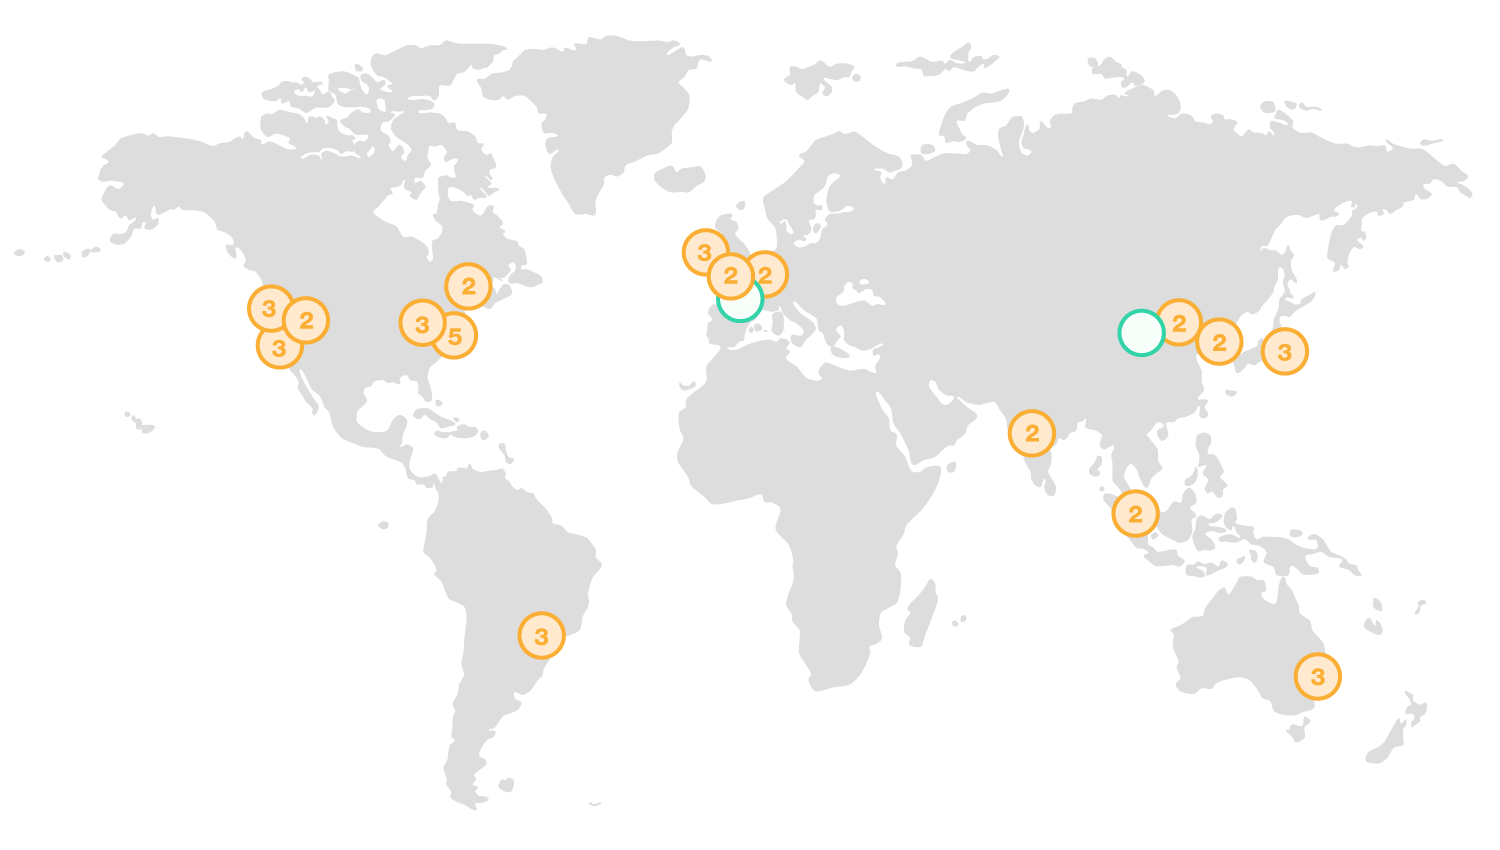
\includegraphics[width=0.9\textwidth]{images/regions.png}
  \caption{weltweite Infrastruktur (orange: Region mit x AZs, weiß/grün: geplante Region) \cite{aws:regions}}
\end{figure}

Eine Region entspricht einem physischen Ort auf der Welt, welcher mehrere Availability Zones (AZs) beherbergen kann. Bei einer AZ handelt es sich um ein oder mehrere unabhängige Rechenzentren, wobei jedes eine redundante Energieversorung, Netzwerk und Konnektivität besitzt.

\begin{figure}[!ht]
  \centering
  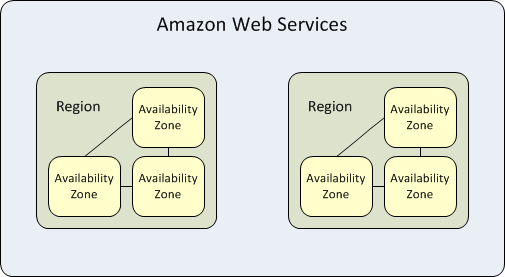
\includegraphics[width=0.7\textwidth]{images/azs_regions.png}
  \caption{Regionen mit zugehörigen Availability Zones \cite{aws:azs}}\label{figure:azs-regions}
\end{figure}

Dies erhöht die Ausfallsicherheit im Falle physischer Schäden z.B. Stürme und ist ein Alleinstellungsmerkmal gegenüber fast allen anderen Anbietern für technologische Infrastrukturen. Es ist daneben auch möglich, Daten zwischen mehreren AZs auszutauschen, um dem Ausfall der Anwendung bei einem Ausfall von AZs in einer Region vorzubeugen. Die AZs sind dafür mit schnellen, privaten Glasfasernetzwerken verbunden.
Durch die Replikation der Daten über mehrere geografische Regionen hinweg, kann die Redundanz und Fehlertoleranz noch zusätzlich erhöht werden.

Die weltweit verteilten Datenzentren sind gerade für international agierende Unternehmen interessant. Je näher ein Datenzentrum dem Endkunden einer Anwendung ist, welche bei AWS gehostet wird, desto geringer fallen die Latenzzeiten aus. Darüberhinaus punktet Amazon mit diesem Konzept beim Thema Datenschutz. In Frankfurt am Main sind 2014 zwei AZs entstanden um Bedenken deutscher Unternehmen hinsichtlich Datenschutz auszuräumen. Kunden können definieren, dass ihre Daten ausschließlich in deutschen Rechenzentren gehalten und bearbeitet werden. Damit unterliegen die dort gehosteten Daten den deutschen Datenschutz-Vorgaben.

Aktuell sind fünf weitere Availability Zones und zwei weitere Regionen geplant.
\\ \cite{computerwoche:reder}, \cite{aws:regions}, \cite{aws:azs}


\section{Vorteile}
\label{sec:vorteile}
Warum ein Einsatz der Amazon Web Services für Unternehmen jeder Größe sinnvoll sein kann, zeigen die Vorteile:
\begin{enumerate}
  \item Kostenersparnis
  \\ An oberster Stelle der Vorteile eines Einsatzes von IT-Ressourcen in der Cloud gegenüber einem klassischen Rechenzentrum stehen die Kosten. Statt einer Aufstellung der IT-Ressourcen für die nächsten Jahre, können Ressourcen bei AWS nach Bedarf beansprucht werden. Ist die Zugriffsrate auf die Webseite gerade sehr hoch, können in wenigen Minuten weitere Server bereitgestellt werden, um die Gesamtlast aufzuteilen. Bezahlt wird dabei nach dem "`Pay-per-use"'-Prinzip. Es werden nur Kosten für Ressourcen erhoben, die auch tatsächlich verwendet wurden.
  \item Hohe Innovations-Geschwindigkeit
  \\ Im Jahr 2015 hat Amazon 722 neue Services und Features umgesetzt. 40\% mehr als im Jahr zuvor. Wöchentlich werden neue Features und Verbesserungen veröffentlicht. Möglich wird das durch viele kleine Teams, die unabhängig voneinander arbeiten. Dabei stehen die Umsetzung der Wünsche der mittlerweile über eine Millionen Kunden im Vordergrund.
  \item Weltweite Infrastruktur
  \\ AWS Nutzer können auf ein Netzwerk weltweit verteilter Datenzentren zurückgreifen. Siehe Sektion \ref{sec:regions}
  \item Arbeitserleichterung
  \\ Auf Wunsch übernimmt AWS mit seinem enormen Dienstangebot notwendige Arbeiten der Nutzer, die sie sonst in Eigenregie erledigen bzw. verwalten müssten. Zum Beispiel Load Balancing zwischen den Servern oder das Aufsetzen eines E-Mail-Service.
  \item Automatisierung
  \\ Viele Dinge, die einen gewissen manuellen Aufwand und ab einer gewissen Komplexität auch eine kognitive Herausforderung bedeuten, können über Skripte automatisiert werden. Via Code können Instanzen aufgesetzt oder Container und Datenbanken bereitgestellt werden. Um Abhängigkeiten muss sich der Anwender dabei nicht sorgen, denn das übernimmt der Computer ganz automatisch. Die Infrastruktur kann beliebig flexibel definiert werden ohne dass manuelle Einstellungen auf der AWS Webseite getätigt werden müssen. Und das Beste daran ist, dass diese Skripte über ein Versionierungs-Tool versioniert werden können und im Fall eines Komplettabsturzes des Systems selbiges in sehr kurzer Zeit neu aufgesetzt werden kann. {\color{red}Vergleich Infrastructure as Code}
  \item Skalierbarkeit
  \\ Neben den Kosten ist Skalierbarkeit wohl das stärkste Argument für eine IT-Infrastruktur in der Cloud. Im Gegensatz zur "`klassischen"' IT, bei der weit in die Zukunft geplant werden und zukünftige Zugriffszahlen abgeschätzt werden mussten, können bei AWS Ressourcen innerhalb von Minuten hinzugeschaltet werden. Sollte der Ansturm vorbei sein und Ressourcen nicht mehr benötigt werden, können diese ebenso schnell wieder abgeschaltet werden, Das ist agil, umweltfreundlich und spart auch noch Geld. Nicht nur zum Auffangen schwankender Zugriffszahlen, auch für das schnelle Bereitstellen von Testsystemen stellt eine hohe Skalierbarkeit der IT-Ressourcen einen großen (Geschwindigkeits-)Vorteil dar.
  \item Ausfallsicherheit
  \\ Die meisten angebotenen Dienste implizieren bereits eine Ausfallsicherheit, so dass sich der Anwender um dieses Problem auch nicht mehr kümmern muss.
  \item Schnelle Anpassungsfähigkeit
  \\ Durch die bereits erwähnte hohe Skalierbarkeit ist auch eine flinke Anpassung an sich ändernde Anforderungen z.B. durch den sich schnell wandelnden Markt gegeben. Entwicklungszyklen können deutlich kürzer ausfallen, da Testsysteme schneller bereitgestellt und Tests schneller durchgeführt werden können.
  \item Die Menge macht's
  \\ Je mehr Kunden AWS nutzen, desto günstiger werden die Dienste für den Einzelnen. Denn um die stetig wachsende Nutzerzahl mit gleichbleibendem Service bedienen zu können, müssen die unterliegenden Prozesse so optimal wie möglich sein.
  \begin{figure}[!ht]
    \centering
    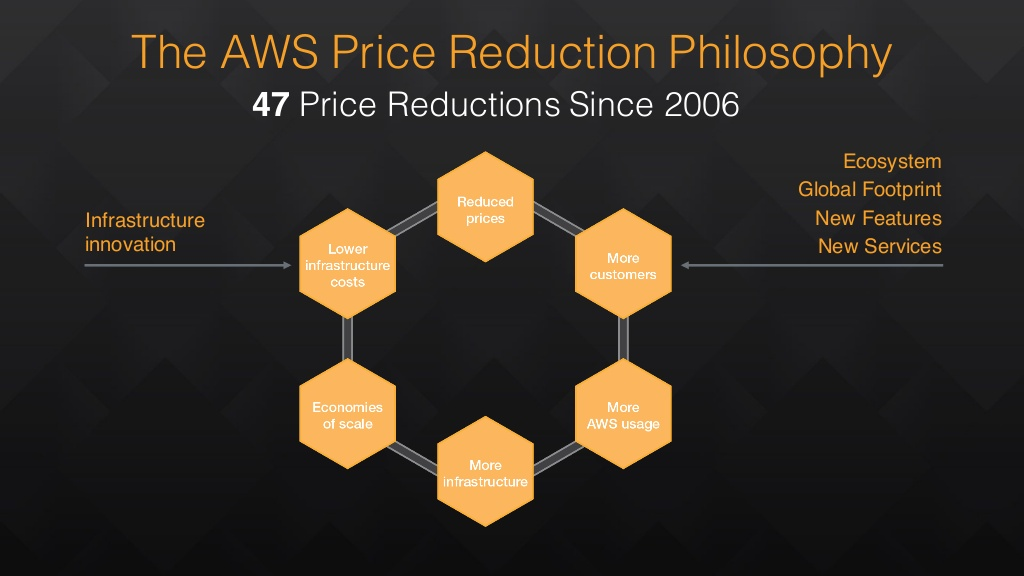
\includegraphics[width=0.9\textwidth]{images/price-reduction.jpg}
    \caption{Preis-Reduktions-Philosophy \cite{aws:insider}}
  \end{figure}
  \item Professionalität
  \\ AWS setzt verschiedene Standards ein, um z.B. Zahlungssicherheit und Datensicherheit zu gewährleisten. Für weitere Informationen zu eingesetzten Standards siehe Kapitel 1.3.9 \cite{wittig:awsinaction})
\end{enumerate} \cite{aws:insider}, \cite{wittig:awsinaction}, \cite{vliet:programmingec2}


\section{Kosten}
Die Kosten für AWS sind abhängig von der Nutzung ("`pay-per-use"'-Prinzip). Zum Beispiel wie viel Speicherplatz verbraucht wird oder wie viel die Laufzeit eines virtuellen Servers beträgt. Dieses Konzept ist gerade für kleine Unternehmen mit einem geringen Budget interessant, da sie weitaus bessere Möglichkeiten haben von Beginn an fehlertolerante Systeme aufzusetzen. Der Betrieb eines großen Servers kostet am Monatsende ebenso viel wie der Betrieb zweier kleinerer Server mit der selben Kapazität wie der große Server. Jedoch bietet die Infrastruktur mit zwei Servern die Möglichkeit redundanter Datenhaltung.
\\Für zukünftig geplante Installationen bietet AWS auf seiner Seite einen Preisrechner \cite{aws:calc}.
\\ Seit 2010 bietet Amazon die Möglichkeit, in begrenztem Maße beliebte Dienste und Rechenleistung (750 Stunden) für 12 Monate kostenlos auszuprobieren. Dieses Programm nennt sich "`Free Usage Tier"'. \cite{wikipedia:aws}, \cite{wittig:awsinaction}

\section{Sicherheit}
Die Sicherheit der eigenen gehosteten Daten ist einer der wichtigsten Punkte, die Amazon gewährleisten muss. Um deutschen Datenschutz- und Datensicherheitsstandards gerecht werden zu können, wurden zwei Datenzentren in Frankfurt am Main eröffnet. Die Daten werden auf Wunsch der Kunden nicht auf amerikanischen Servern gespiegelt und es steht Entwicklern ausdrücklich frei, die hinterlegten Daten zu verschlüsseln. Allerdings war in der Vergangenheit auch immer wieder von Sicherheitslücken die Rede und auch die Auftragsvergabe einer public cloud der CIA an Amazon wurde hinsichtlich des Datenschutzes kritisch beurteilt \cite{computerwoche:sicherheit}, \cite{sueddt:cia}.

% keep an blank line above
